\documentclass[10pt]{article}
\usepackage[accepted,preprint]{tmlr}
\usepackage{amsmath,amssymb}
\usepackage{booktabs}
\usepackage{graphicx}
\usepackage{hyperref}
\usepackage{url}
\hypersetup{hidelinks}

\def\month{09}
\def\year{2026}

\title{What Does a Benign-Trained Anomaly Detector Actually Detect?}

\author{\name Suramya Angdembay \email suramya.angdembay@usm.edu \\
\addr University of Southern Mississippi
\AND
\name Haiyan Tian \email haiyan.tian@usm.edu \\
\addr University of Southern Mississippi}

\begin{document}
\maketitle

\begin{abstract}
Anomaly detectors for insider threats are usually judged by how well
their scores rank malicious activity above normal activity. We show that
this number can be misleading, because it does not reveal what
information the detector uses. We build a detector by adapting a large
language model to normal employee activity only, so that unusual
activity receives a high surprisal score, and we then open the model to
determine what its score is based on: we isolate the internal changes
that adaptation caused, approximate them with a sparse dictionary, test
which dictionary directions causally influence the score, and measure
what part of the input those directions respond to. On one standard
benchmark the score turns out to rest almost entirely on who each user
is (their recorded personality and organizational profile) rather than
on what they did; on a second benchmark the score rests mostly on
behavior. When malicious users are compared only against normal users
that the model has never seen, apparent ranking quality falls from about
$0.95$ to near chance on the first benchmark. The finding survives an
extensive robustness program: held-out users, repeated dictionary
training, dictionaries trained without any malicious example, a smaller
model retrained from scratch with fresh random seeds and a repaired data
pipeline, and interventions whose strength is matched between treatment
and control. The same analysis on a third dataset, collected from real
people with real personality questionnaires, confirms the behavioral
case, and classical statistical detectors trained on the same
information do not take the profile shortcut. The conclusion is that
high ranking performance alone does not show that a detector has learned
to detect behavior, and this paper provides a way to check.
\end{abstract}

\section{The problem}

Organizations record what employees do on their computers: logons, file
transfers, web activity, e-mail volume, and so on. An \emph{insider
threat} is an employee who misuses legitimate access, for example by
stealing data. Because such events are rare, a common approach is
\emph{anomaly detection}: build a statistical model of normal activity,
and flag days that the model finds unusual.

Formally, a detector is a function $s$ that assigns a real-valued
\emph{anomaly score} $s(x)$ to each observation $x$, where in our
setting $x$ is a record of one user's activity on one day. Higher
scores are meant to indicate more suspicious activity. Detectors are
usually evaluated by how well their scores \emph{rank} malicious days
above benign ones. The standard summary of ranking quality is the
following probability, estimated over a labeled test set:
\begin{equation}
\mathrm{AUC} \;=\; \Pr\bigl( s(X_{\mathrm{mal}}) > s(X_{\mathrm{ben}})
\bigr),
\label{eq:auc}
\end{equation}
where $X_{\mathrm{mal}}$ is a randomly chosen malicious day and
$X_{\mathrm{ben}}$ a randomly chosen benign day. (This quantity is
commonly called the ROC-AUC, for ``area under the receiver operating
characteristic curve''; the probability formulation is equivalent and is
the only form we need.) An AUC of $1$ means perfect ranking and $0.5$
means the ranking is no better than chance.

The question that motivates our work is simple to state. A high AUC
says that the score \emph{separates} the two classes. It does not say
\emph{on the basis of what information} the separation is achieved. Two
detectors with identical AUC could work very differently: one might
respond to genuinely unusual behavior, while the other might respond to
incidental properties of \emph{who} the malicious users happen to be,
such as their role, department, or personality profile. The second kind
of detector would be nearly useless in practice, because in deployment
the malicious users are not known in advance. This paper develops a
method for determining which kind of detector one actually has, applies
it to a modern detector built from a large language model, and then
subjects the answer to a systematic robustness program.

\section{The data}
\label{sec:data}

We use two versions (called r4.2 and r6.2) of the CERT insider-threat
corpus, a widely used synthetic dataset that simulates a corporation's
activity logs, produced by Carnegie Mellon University. Each version
contains several thousand simulated employees observed over about
eighteen months, with a small set of employees scripted to carry out
malicious scenarios on particular days. Version r4.2 has sixty
malicious users among about one thousand; version r6.2 has four among
about four thousand. This difference in composition turns out to
matter, and we return to it repeatedly. A third dataset, TWOS,
collected from real people, is described in
Section~\ref{sec:twos}.

Each user-day is converted into a short structured text with three
kinds of lines:
\begin{itemize}
\item a \texttt{DAY} line holding static organizational fields for that
user (project, role, business unit, department, team, and an
information-technology administrator flag);
\item a \texttt{PSY} line holding the user's five simulated personality
scores. These are the ``Big Five'' personality traits used in
psychology: openness (O), conscientiousness (C), extraversion (E),
agreeableness (A), and neuroticism (N). In CERT these numbers are
generated by the simulator and are constant for each user;
\item one \texttt{SES} line per work session, holding numeric
behavioral counts for that session: duration, number of logons, file
and removable-drive activity, e-mail volume, web-browsing category
counts, and similar quantities.
\end{itemize}
A user-day text is therefore a small table serialized as text. The
first two lines describe \emph{who the user is} and are essentially
constant across a user's days; the remaining lines describe \emph{what
the user did} that day. We call the first two line classes
\emph{profile} content and the third \emph{behavioral} content. This
partition of the input is the reference frame for the entire paper.

Users are split as follows. Users with any malicious day are reserved
entirely for evaluation. The remaining benign users are divided into a
training set (roughly ninety percent) and a validation set (roughly ten
percent) whose days never enter training. The validation users will
play an important role: they are the only benign users about whom the
trained model knows nothing.

\section{The detector}
\label{sec:detector}

\subsection{Language models as probability distributions}

A \emph{language model} is a parametric probability distribution over
sequences of symbols called tokens. Writing a sequence as
$x = (x_1, \dots, x_n)$, the model has the product form
\begin{equation}
p_\theta(x) \;=\; \prod_{t=1}^{n} p_\theta\bigl(x_t \mid x_1, \dots,
x_{t-1}\bigr),
\end{equation}
where each conditional distribution is computed by a neural network
with parameters $\theta$. Modern large language models are such
networks with billions of parameters, trained on enormous general text
corpora. We use one called Qwen3-8B (eight billion parameters). The
network processes a sequence through $L$ successive layers; at layer
$\ell$ and position $t$ it maintains an internal state vector
$h^{(\ell)}_t \in \mathbb{R}^{d}$ with $d = 4096$. These internal
vectors matter later: they are the objects we analyze.

\subsection{Adapting the model to normal behavior only}

We specialize the general-purpose model to our corpus by
\emph{fine-tuning}: continuing its training on the serialized user-day
texts, using only days from benign training users. The objective is
maximum likelihood, that is, minimizing the negative log-likelihood of
the benign corpus $\mathcal{D}$:
\begin{equation}
\mathcal{L}(\theta) \;=\; -\sum_{x \in \mathcal{D}} \sum_{t}
\log p_\theta\bigl(x_t \mid x_{<t}\bigr).
\end{equation}
No malicious example is ever used in training. This is the classical
one-class setup: model the normal population, then measure deviation
from it.

For efficiency the fine-tuning does not modify all eight billion
parameters. Each weight matrix $W$ of the network is kept fixed and
receives a trainable low-rank correction,
\begin{equation}
W' \;=\; W + \tfrac{\alpha}{r} BA, \qquad
B \in \mathbb{R}^{d_{\mathrm{out}} \times r},\;
A \in \mathbb{R}^{r \times d_{\mathrm{in}}},
\end{equation}
with rank $r = 16$, so only the small matrices $A$ and $B$ are learned.
This technique is called LoRA (low-rank adaptation); we use a
memory-saving variant called QLoRA in which the fixed weights are
stored at reduced numerical precision. The pair (fixed base model,
learned low-rank correction) is called the \emph{adapted model}. The
important point is that the entire effect of training is carried by a
low-dimensional, removable perturbation, which makes before-versus-after
comparisons clean.

\subsection{The anomaly score and two ways to evaluate it}
\label{sec:protocols}

The score of a day $x$ is its average surprisal under the adapted
model:
\begin{equation}
s(x) \;=\; -\frac{1}{n}\sum_{t=1}^{n} \log
p_{\theta_{\mathrm{ada}}}\bigl(x_t \mid x_{<t}\bigr).
\end{equation}
Days that the model of normal behavior finds improbable receive high
scores.

There are two reasonable ways to estimate the AUC of
equation~\eqref{eq:auc}, and the difference between them will turn out
to be one of the paper's findings.
\begin{enumerate}
\item \emph{The standard protocol.} Malicious days are compared against
benign days drawn from the general population. Because the model was
trained on about ninety percent of benign users, most of those benign
comparison days belong to users the model saw during training. Under
this protocol the adapted model looks excellent: AUC about $0.953$ on
r6.2 and $0.964$ on r4.2, higher than four standard anomaly-detection
baselines evaluated on the same benchmarks (an isolation forest, a
one-class support vector machine variant called Deep SVDD, and two
recurrent autoencoders), whose AUC values range from about $0.63$ to
$0.77$.
\item \emph{The user-disjoint protocol.} Malicious days are compared
only against benign days of the validation users, whom the model never
saw. Malicious users are unseen by construction, so under this protocol
both sides of the comparison are equally unfamiliar to the model.
\end{enumerate}
The gap between these two numbers measures how much of the apparent
performance is explained by mere familiarity with specific users rather
than by properties of the activity itself. We report the gap in
Section~\ref{sec:collapse}.

\section{Opening the model}
\label{sec:method}

We now describe the four analysis steps, in the order they are applied.
Together they take us from the raw network to a statement about what
the score is based on.

\subsection{Step 1: isolate what fine-tuning changed}

Because the base model is kept frozen, we can run the same day $x$
through both the base and adapted models and subtract their internal
states. Define, at a chosen layer $\ell$ and each token position $t$,
\begin{equation}
\delta_t \;=\; h^{(\ell), \mathrm{ada}}_t - h^{(\ell),
\mathrm{base}}_t \;\in\; \mathbb{R}^{d}.
\end{equation}
The vector $\delta_t$ isolates the representational change induced by
the adaptation at the audited layer and position. It is the natural
object to study if one wants to know what the adaptation, as opposed to
the general-purpose model, contributes at that point in the
computation.

\subsection{Step 2: approximate the changes with a sparse dictionary}

The vectors $\delta_t$ live in $\mathbb{R}^{4096}$ and are not
individually interpretable. We therefore approximate them by sparse
nonnegative combinations of learned dictionary elements. After
standardizing each coordinate (subtracting its mean $\mu$ and dividing
by its standard deviation $\sigma$), we seek a dictionary matrix
$D \in \mathbb{R}^{d \times m}$ (with $m = 4d$ columns, called
\emph{features}) and, for each standardized vector
$\tilde\delta_t$, a coefficient vector
$z_t \in \mathbb{R}^{m}_{\geq 0}$ with at most $k = 8$ nonzero
entries, such that
\begin{equation}
\tilde\delta_t \;\approx\; D z_t ,
\end{equation}
with $D$ and the coefficients chosen to minimize the mean squared
reconstruction error over a large sample of token positions. This is a
sparse coding problem; the particular parametrization we use (a
one-layer encoder network followed by a keep-the-largest-$k$ rule and a
linear decoder) is called a \emph{sparse autoencoder} in the
machine-learning literature. The outcome is that each change vector is
expressed as a short combination of reusable directions, and each
direction can be studied on its own. One technical point deserves
notice: because the standardization constants differ between datasets,
any geometric comparison of features across datasets must first map the
dictionary columns back to the original coordinates, that is, compare
the directions $\sigma \odot D_{:,f}$ rather than the raw columns. All
cross-dataset comparisons in this paper do so.

\subsection{Step 3: select the score-relevant features and test them
causally}
\label{sec:interventions}

Some dictionary features activate similarly on malicious and benign
days; those cannot carry the anomaly signal. We rank features by the
difference in mean activation,
\begin{equation}
g_f \;=\; \mathbb{E}\bigl[z_{t,f} \mid \text{malicious day}\bigr] -
\mathbb{E}\bigl[z_{t,f} \mid \text{benign day}\bigr],
\end{equation}
and take the five features with the largest $g_f$ as the candidate set
$S$. As a comparison group we also select a matched \emph{control} set
$C$ of five features that are similarly active overall but carry no
class difference (small $|g_f|$). Selection by a statistic can be
flattered by chance, so everything that follows treats $S$ as a
hypothesis to be tested rather than a conclusion.

The test is interventional. The idea is to edit the coefficients of the
selected features inside the model, let the edited internal state flow
through the remaining layers, and observe whether the anomaly score
responds. We use two complementary edits.

\emph{Repair (a sufficiency-style test).} For a malicious day, we move
the selected coefficients toward the values they take on a comparable
benign day (a ``donor'' from the same organizational context, never the
same user), with an interpolation strength
$\alpha \in \{0.25, 0.5, 0.75, 1\}$, and record the best achievable
reduction of the score over the available donors and strengths. Write
$\Delta^{S}_{\mathrm{ben}}$ for this quantity, and
$\Delta^{S}_{\mathrm{anom}}$ for the analogous quantity when donors are
other malicious days. If the selected features carry anomaly-specific
repairable structure, moving them toward benign values should reduce
the score more than moving them toward other anomalous values, and it
should do so more for $S$ than for the control set $C$. The reported
estimand is the doubly differenced quantity
\begin{equation}
\tau \;=\; \bigl(\overline{\Delta^{S}_{\mathrm{anom}}} -
\overline{\Delta^{S}_{\mathrm{ben}}}\bigr) -
\bigl(\overline{\Delta^{C}_{\mathrm{anom}}} -
\overline{\Delta^{C}_{\mathrm{ben}}}\bigr).
\end{equation}
The double difference protects the comparison: any effect that comes
merely from making a large edit, rather than from the specific content
of the selected features, appears in both arms and cancels at the level
of the contrast.

\emph{Ablation (a necessity-style test).} We scale the selected
coefficients toward zero, on malicious days and on matched benign days,
and ask whether removal disrupts the score more on the malicious side
and more for $S$ than for $C$. The corresponding double difference is
denoted $\nu$.

Two safeguards are essential and were arrived at the hard way. First,
donors from the same user are excluded: allowing them lets the
procedure ``repair'' a malicious day by borrowing the same person's own
benign signature, which inflates effects for reasons unrelated to the
question. Second, uncertainty is computed by resampling \emph{users},
not days: multiple days of the same user are statistically dependent,
so all confidence intervals in this paper are user-level bootstrap
intervals with the malicious user as the resampling unit ($10{,}000$
draws). On r6.2, which has only four malicious users, such intervals
are reported as descriptive.

One further check matters because the selected features are, by
construction, strongly activated: their edits are physically larger
than edits of the control features. We therefore repeated the headline
comparisons with \emph{dose-matched} controls, chosen to match the
selected features on activation frequency, activation magnitude, and
dictionary-direction norm, which closes the edit-size gap to a factor
of $1.3$ to $1.8$. The contrasts survive: on r4.2 the repair contrast
remains clearly positive ($+0.0017$ with interval $[0.0011, 0.0023]$)
and on r6.2 the ablation contrast remains clearly positive ($+0.061$
with interval $[0.007, 0.084]$); the remaining two contrasts stay
positive but with intervals containing zero. Figure~\ref{fig:effects}
summarizes the intervention measurements.

\begin{figure}[t]
\centering

\includegraphics[width=\textwidth]{figures/mech_effects.pdf}
\caption{Effect of editing the selected features, compared with editing
matched control features, on the anomaly score (one panel per benchmark
and per type of edit; units are thousandths of the score). Each point
is the average effect for one organizational matching context, and each
horizontal bar is a $95$ percent confidence interval computed with the
malicious users as the resampling unit. Positive values mean that the
selected features influence the score more strongly than the control
features do. Open circles mark intervals that include zero.}
\label{fig:effects}
\end{figure}

\subsection{Step 4: read off what the features respond to}

Finally we ask \emph{where} the selected features activate within the
day text. Every token position belongs to one line class: the
organizational \texttt{DAY} line, the personality \texttt{PSY} line, or
a behavioral \texttt{SES} line. For a feature $f$, define its
\emph{attribution mass} on class $c$ as the fraction of its total
activation that occurs at positions of that class:
\begin{equation}
m_f(c) \;=\;
\frac{\sum_{(x,t)\,:\, \mathrm{class}(t) = c} z_{t,f}(x)}
     {\sum_{(x,t)} z_{t,f}(x)} .
\end{equation}
If a feature has nearly all of its mass on \texttt{PSY} and
\texttt{DAY} positions, it responds to who the user is; if its mass
lies on \texttt{SES} positions, it responds to what the user did.

The logic of the whole method is a conjunction. The interventions of
Step~3 establish that the selected features are causally connected to
the score, but say nothing about their meaning. The attribution of
Step~4 establishes what the features respond to, but says nothing about
whether they matter. Only together do the two steps answer the question
in the title, and the paper's findings repeatedly illustrate that
either step alone would have been misleading.

\section{Findings on the two CERT benchmarks}
\label{sec:findings}

\subsection{Two detectors that look alike and are not}

The two CERT versions produce nearly identical headline AUC values, yet
the analysis reveals qualitatively different detectors.

On r6.2, the five selected features place between $99.8$ and $100$
percent of their attribution mass on the personality and organizational
lines, with activation on the personality line enriched about thirteen
times over its share of tokens. The intervention contrasts are positive
(repair $\tau = 0.0068$ with descriptive interval $[0.0001, 0.0100]$;
ablation $\nu = 0.065$ with interval $[0.026, 0.083]$). The detector's
causally relevant evidence is almost entirely a description of \emph{who
the user is}.

On r4.2, four of the five selected features concentrate on the
behavioral session lines (the fifth responds to the organizational
header). The contrasts are again positive (repair $\tau = 0.0014$ with
interval $[0.0010, 0.0019]$; ablation $\nu = 0.0029$ with interval
$[0.0009, 0.0050]$). There, the evidence is mostly \emph{what the user
did}. Figure~\ref{fig:attribution} shows the contrast, together with
the real-data result of Section~\ref{sec:twos}.

\begin{figure}[t]
\centering
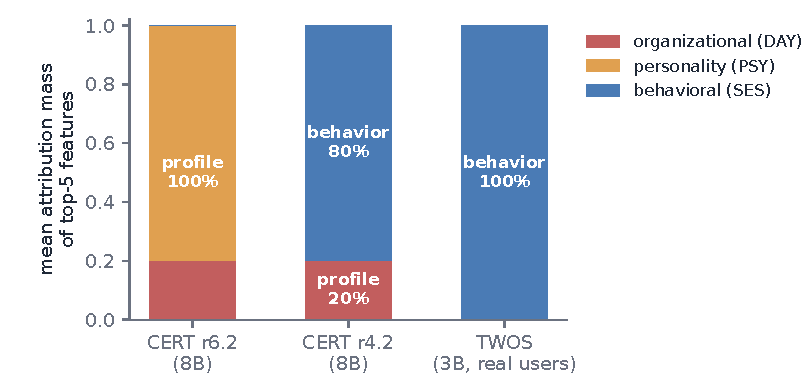
\includegraphics[width=0.85\textwidth]{figures/attribution_summary.pdf}
\caption{Where the selected features place their activation, averaged
over each detector's five selected features. Each bar decomposes the
activation mass into the organizational lines, the personality lines,
and the behavioral session lines of the input text. The r6.2 detector's
evidence is almost entirely a description of who the user is; the r4.2
and TWOS detectors' evidence is almost entirely a description of what
the user did.}
\label{fig:attribution}
\end{figure}

\subsection{The consequence for the headline numbers}
\label{sec:collapse}

Why would reading a user's static profile produce a high AUC at all?
The adapted model was trained on roughly ninety percent of the benign
users. For those users, the model has been repeatedly exposed to the
constant profile lines, so their profile text is comparatively familiar
and their days look unsurprising. The malicious users were never seen
in training, so their profile lines alone make their days look
surprising. The score is then partly measuring \emph{familiarity}
rather than behavior.

The user-disjoint protocol of Section~\ref{sec:protocols} removes this
asymmetry, and the effect is large. The AUC falls from $0.954$ to
$0.545$ on r6.2, which is barely better than chance, and from $0.959$
to $0.668$ on r4.2. Under the fair comparison the language model no
longer outperforms the classical baselines at all. Two further
measurements complete the picture. First, ranking each malicious user's
own days (their malicious days against their own benign days, identity
held fixed) still succeeds moderately on both benchmarks (average
within-user AUC $0.67$ on r4.2 and $0.73$ on r6.2), so behavioral
signal exists; it is simply drowned, in the cross-user comparison, by
the familiarity effect. Second, deleting the personality lines from the
inputs at scoring time \emph{improves} the r4.2 detector's performance
on unseen users from $0.67$ to about $0.80$ (an increase of $0.127$
with interval $[0.061, 0.193]$): the profile text was not merely
unhelpful, it was actively obscuring the behavioral signal. On r6.2,
deleting profile content changes nothing that is statistically
distinguishable; with every user unseen, profile novelty separates
nothing, and no clear behavioral signal is revealed underneath.
Figure~\ref{fig:collapse} shows the baseline comparison and the
collapse.

\begin{figure}[t]
\centering

\includegraphics[width=\textwidth]{figures/detector_dissociation.pdf}
\caption{Score-level results. Left and center panels: ranking quality
(vertical axis) and precision (horizontal axis, logarithmic scale) for
the language-model detector (blue) and four standard anomaly-detection
methods on the two benchmarks; the language model attains the highest
ranking quality under the standard protocol. Right panel: the same
language-model ranking quality when malicious users are compared only
against benign users never seen during training. The apparent advantage
largely disappears, and the dashed line marks chance level.}
\label{fig:collapse}
\end{figure}

\section{Is the interpretation robust?}
\label{sec:robustness}

A single analysis pipeline contains many arbitrary choices, and each is
an opportunity for an artifact. This section walks through the checks,
one question at a time. Each check either survived or, where it did
not, the failure is reported and incorporated into the claims.

\emph{Does the finding survive on users that played no role in
selecting the features?} On r4.2 we split the sixty malicious users
into two halves, re-selected features using only the first thirty, and
estimated effects only on the second thirty. Four of the five selected
features reappear, and all effect estimates remain positive on the
held-out half, at roughly half the original magnitude, with one
matching context individually excluding zero. The shrinkage is the
expected signature of selection effects, and the claims are scoped
accordingly. On r6.2, with only four malicious users, we used
leave-one-user-out selection instead; there the effects concentrate on
the single dominant user, who contributes $46$ of the $70$ malicious
days, and the paper reports r6.2 causal claims at that resolution.

\emph{Is the dictionary itself an accident of its random
initialization?} Training the dictionary three times with different
random seeds and comparing the resulting feature directions (in
original coordinates, as noted in Step~2) shows that each benchmark's
selected feature family is stable: matched features across seeds align
with cosine similarity $0.81$ to $0.95$, above a null baseline of
$0.72$ to $0.82$ computed from the full dictionaries. Across
benchmarks, by contrast, the selected features align at or below the
null; notably, where the two dictionaries share the most overall
geometry, the selected features align \emph{worse} than typical
features. The two detectors' evidence is not the same structure under
different labels.

\emph{Does the finding depend on malicious examples having shaped the
dictionary?} The dictionaries above were fitted on a pool that includes
malicious days. We retrained both dictionaries from scratch on benign
rows only, so that no malicious example influences dictionary
formation, and repeated selection, attribution, and evaluation. The
attribution dissociation reproduces exactly (r4.2 selected features at
least $94$ percent behavioral; r6.2 features at least $99$ percent
profile-bound in every leave-one-user-out fold). The intervention
results are estimand-dependent under the new dictionaries: the ablation
contrast on r4.2 replicates across all matching contexts, while the
repair contrast does not. We therefore treat ablation dependence as the
robust causal signature and report repair effects with that
qualification.

\emph{Is the difference between the benchmarks simply that one has four
malicious users and the other sixty?} We subsampled r4.2's malicious
population down to four users (ten random repetitions per size) and
re-ranked features each time. The profile share of the selected
features stays low and nearly flat across population sizes. Raw
positive count alone does not explain the dissociation; the composition
of the population, not its size, is what matters.

\emph{Does the finding survive a fresh model, fresh randomness, and a
repaired pipeline?} A data-serialization defect (four file-transfer
fields silently dropped) was discovered during the project. We repaired
it and reran the entire pipeline at smaller scale: a different, smaller
language model (Qwen2.5-3B) trained from scratch twice per benchmark
with different random seeds, new dictionaries trained on benign rows
only, and fresh selection and attribution. The dissociation reproduces
under both seeds: r4.2 selected features are behavioral in every
audited configuration, and r6.2 develops features that are $100$
percent profile-bound at the deepest audited layer under both seeds.
The ablation contrast again replicates on r4.2 across seeds
($+0.0022$ and $+0.0021$) while the repair contrast again does not,
matching the pattern above.

\emph{Could the score's profile sensitivity be an illusion of the
analysis rather than a property of the score?} Two input-level
experiments require no interpretability machinery at all and agree with
the internal analysis. Replacing a malicious day's profile lines with a
random benign user's profile changes the r6.2 score substantially,
while replacing its entire behavioral content changes it much less; on
r4.2 the sensitivities are reversed. And the masking result of
Section~\ref{sec:collapse} shows the score-level consequence directly.

\section{Real data with real personality scores}
\label{sec:twos}

The CERT data are simulated, including the personality scores. The
natural objection is that the entire phenomenon might be an artifact of
simulation. We therefore repeated the pipeline on TWOS, a public
dataset collected at the Singapore University of Technology and Design
from twenty-four real users over one week, during which, by design of
the underlying study, twelve users had their sessions temporarily taken
over by other participants (a ``masquerade'' attack). Each real user
completed the standard fifty-item Big Five questionnaire, so the
serialized inputs contain genuine psychometric information.

The details mirror the CERT setup at smaller scale. Mouse, keyboard,
and logon telemetry are aggregated into ten-minute windows and
serialized in the same three-line-class format, with the real Big Five
scores forming the personality line ($18{,}048$ windows in total, of
which $138$ overlap a staged attack). The model is the smaller
Qwen2.5-3B, adapted on benign users' windows only (about seven thousand
windows from the twelve never-attacked users), trained twice with
different random seeds; dictionaries are trained on benign rows only;
selection and attribution proceed exactly as before.

Because half of the users are attacked, profile information is a far
weaker separator here than in CERT r6.2, and our account predicts that
the detector should rely on behavior. That is what the analysis finds.
The selected features place essentially all of their attribution mass
on the behavioral lines, under both training seeds and at both audited
layers (the smallest behavioral share of any selected feature is
$0.983$). Decisively, the evaluation compares each attacked user's
attack windows with that same user's normal windows, so static identity
and personality information is held fixed and cannot explain the
observed separation; the average within-user AUC is $0.78$ across the
sixteen attacked users. The intervention experiments reproduce the
pattern seen on CERT: the ablation contrast is positive
($+0.0019$) while the repair contrast is not, the fourth independent
occurrence of that asymmetry. The behavioral pole of the dissociation
is not an artifact of synthetic data or simulated psychometrics.

\section{Which detectors take the shortcut?}
\label{sec:classical}

One further question separates two very different readings of the r6.2
result. Is the profile information so predictive in that dataset that
\emph{any} statistical method would exploit it, or is the shortcut a
property of this particular detector's construction?

To answer it we trained three classical anomaly detectors on the same
r6.2 days, represented as ordinary numeric feature vectors that
\emph{include} the profile variables (twelve profile columns among
$242$ behavioral ones): an isolation forest, a one-class support vector
machine, and a principal-component reconstruction method, each trained
only on benign training users and evaluated user-disjointly, exactly as
the language model was. For attribution we use permutation importance,
which is defined without reference to any particular model class: for
each input column, randomly permute that column's values across the
evaluation days, recompute the AUC, and record the decrease; the
importance of a group of columns is its share of the total decrease.

All three classical detectors essentially ignore the profile variables.
The profile columns receive four to seven percent of the total
importance, no profile column appears among any detector's five most
important columns, and deleting the profile columns entirely does not
reduce any detector's AUC (it slightly increases it, by $0.003$ to
$0.022$). The same holds on r4.2. The shortcut is therefore not an
inevitable consequence of the available profile information: we do not
observe comparable profile reliance in the three classical baselines.
An explanation consistent with this evidence lies in the training
objective. For a likelihood-based sequence model, the per-user-constant
profile tokens are the most predictable part of every training
sequence, so learning them yields a large and cheap reduction of the
training loss; in a plain feature-vector representation the same
information is twelve columns among $242$, with no comparable incentive
attached. This also explains a number from
Section~\ref{sec:collapse}: under the fair protocol the language model
\emph{underperforms} the classical baselines on r6.2, exactly as
expected if its adaptation spent capacity on a shortcut that does not
generalize while the baselines learned behavior.

\section{Conclusions}
\label{sec:conclusions}

The overall picture can be stated as a two-factor account. The
composition of a dataset's malicious population determines \emph{when}
an identity shortcut is available: profile information separates the
classes when the malicious users are a small, distinctive minority
(CERT r6.2) and separates nothing when they are not (TWOS). The
training objective and input representation determine \emph{which}
detectors take an available shortcut: the likelihood-based sequence
model took it, and three classical feature-vector detectors did not.
Both factors were tested rather than assumed: the first by subsampling
and by an out-of-setting prediction that the real-user dataset
confirmed, the second by the cross-detector comparison.

Three practical conclusions carry beyond these datasets and this
model. First, for anomaly detectors intended to detect behavior,
ranking quality alone is not evidence of success; evaluation should
compare malicious observations only against normal observations from
equally unseen users, and, where possible, within users. Second,
including static descriptors of people (role, department, personality
measures) in a detector's input is not harmless; here it created the
shortcut in one detector and degraded performance even where the
detector was behavioral. Third, the question ``what does this detector
actually detect?'' is answerable: differences of internal states, a
sparse dictionary approximation, causal testing of selected directions
against matched controls, and attribution of those directions to input
content jointly turn the question into a measurable quantity, and the
robustness program of Section~\ref{sec:robustness} is what entitles the
answer to be believed.

The claims are scoped by design. The causal results concern the
particular adaptation runs audited here; the r6.2 estimates rest on
four malicious users dominated by one; the CERT data are synthetic; and
the real-data study is small. What survives every variation we tested
is the central dissociation and its explanation, and the method by
which both were found.

\end{document}
